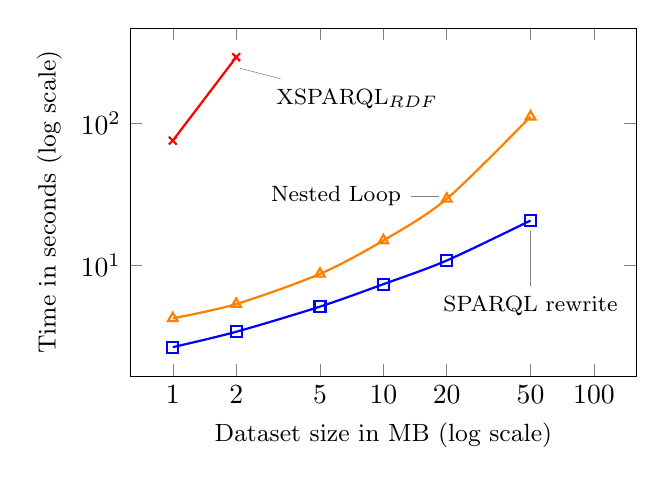
\begin{tikzpicture}[
]\begin{loglogaxis}[
xlabel={{\small Dataset size in MB (log scale)}},
ylabel={{\small Time in seconds (log scale)}},
scaled x ticks = false,
x tick label style = {/pgf/number format/fixed},
scaled y ticks = false,
y tick label style = {/pgf/number format/fixed},
xmax=100,enlargelimits=true,xtick={1,2,5,10,20,50,100},xticklabels={1,2,5,10,20,50,100},log basis x=10,log basis y=10,unbounded coords=jump,xminorticks=false,yminorticks=false,height=6cm,width=8cm,filter discard warning=false,legend style={inner sep=0,legend columns=2,draw=none,font=\tiny,at={(0,0)},anchor=south east,legend pos=south east,anchor=south east,legend cell align=left},pin distance=1em]


\addplot[thick,smooth,color=red, every mark/.append style={solid},mark=x, every pin/.append style={solid},] coordinates {
(1.0000000000, 75.9650000000)
(2.0000000000, 293.6200000000)
(5.0000000000, inf)
(10.0000000000, inf)
(20.0000000000, inf)
(50.0000000000, inf)
(100.0000000000, inf)
} node[pos=.9,pin=-20:{\color{black}{{\footnotesize XSPARQL${}_{RDF}$}}}] {};
\addplot[thick,smooth, color=orange, every mark/.append style={solid},mark=triangle,] coordinates {
(1.0000000000, 4.2662500000)
(2.0000000000, 5.3737500000)
(5.0000000000, 8.7637500000)
(10.0000000000, 15.0550000000)
(20.0000000000, 29.5687500000)
(50.0000000000, 112.0800000000)
(100.0000000000, NaN)
} node[pos=.7,pin=180:{{\footnotesize \color{black}{Nested Loop}}}] {};

\addplot[thick,smooth, color=blue, every mark/.append style={solid},mark=square,pin distance=2em] coordinates {
(1.0000000000, 2.6725000000)
(2.0000000000, 3.4300000000)
(5.0000000000, 5.1550000000)
(10.0000000000, 7.4162500000)
(20.0000000000, 10.8837500000)
(50.0000000000, 20.8087500000)
(100.0000000000, NaN)
} node[pos=1,pin=-90:{\color{black}{{\footnotesize SPARQL rewrite}}}] {};


\end{loglogaxis}\end{tikzpicture}


%%% Local Variables:
%%% mode: latex
%%% mode: flyspell
%%% mode: reftex
%%% TeX-master: "../../presentation"
%%% End:
